
\begin{figure}
	\centering
	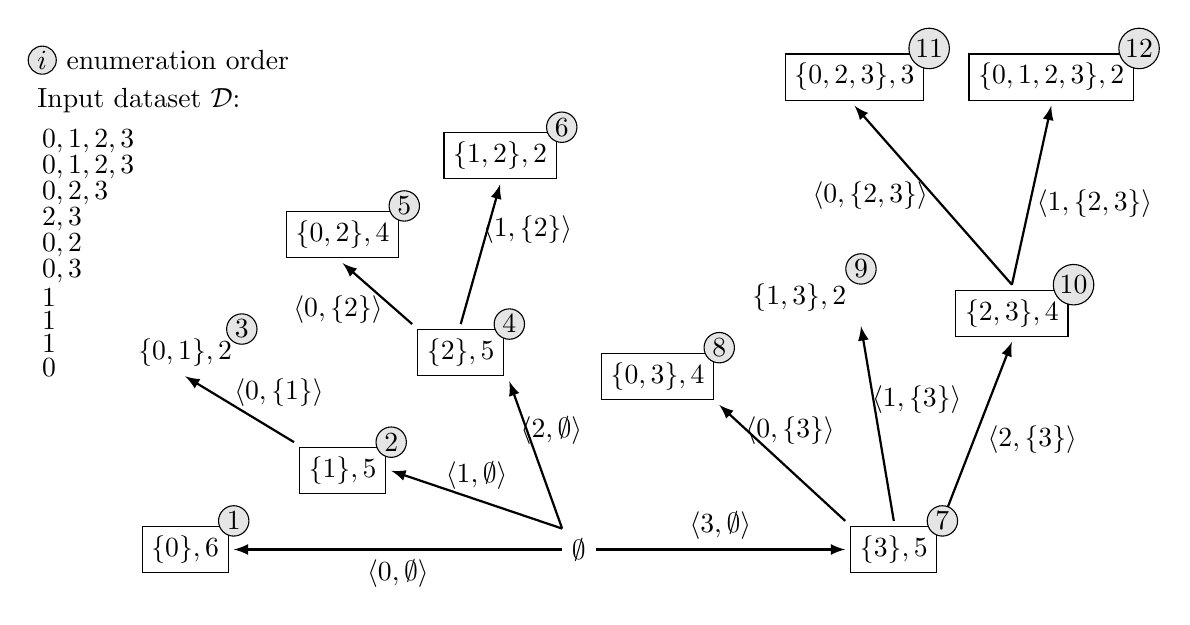
\begin{tikzpicture}[>=latex]%[>=triangle 45]
		\node[inner ysep=1em,anchor=west] (t0) at (-7,5.7) {Input dataset $\cal D$:};
		\node[inner sep=0.5em,anchor=west] (t1) at (t0.south west) {$0, 1, 2, 3$};
		\node[inner sep=0.5em,anchor=west] (t2) at (t1.south west) {$0, 1 , 2, 3$};
		\node[inner sep=0.5em,anchor=west] (t3) at (t2.south west) {$0, 2, 3$};
		\node[inner sep=0.5em,anchor=west] (t4) at (t3.south west) {$2, 3$};
		\node[inner sep=0.5em,anchor=west] (t5) at (t4.south west) {$0, 2$};
		\node[inner sep=0.5em,anchor=west] (t6) at (t5.south west) {$0, 3$};
		\node[inner sep=0.5em,anchor=west] (t7) at (t6.south west) {$1$};
		\node[inner sep=0.5em,anchor=west] (t8) at (t7.south west) {$1$};
		\node[inner sep=0.5em,anchor=west] (t9) at (t8.south west) {$1$};
		\node[inner sep=0.5em,anchor=west] (t10) at (t9.south west) {$0$};

		\node (legenC)[draw,circle,fill=gray!20,inner sep=1pt,anchor=west] at (t0.north west) {$i$};
		\node [right] at (legenC.east) {enumeration order};



		\node (empty) at (0,0) {$\emptyset$};

		\node (0)     [draw,outer sep=2pt] at (-5,0) {$\{0\},6$};
		\node (s0)    [draw,circle,fill=gray!20,inner sep=1pt] at (0.north east) {1};
		\draw [->,thick] (empty.west) -- (0.east) node[below, midway] {$\langle 0, \emptyset\rangle$};

		\node (1)     [draw,outer sep=2pt] at (-3,1) {$\{1\},5$};
		\node (s1)    [draw,circle,fill=gray!20,inner sep=1pt] at (1.north east) {2};
		\draw [->,thick] (empty.north west) --(1.east) node[above, midway] {$\langle 1, \emptyset\rangle$};

		\node (01)     at (-5,2.5) {\st{$\{0,1\},2$}};
		\node (s01)    [draw,circle,fill=gray!20,inner sep=1pt] at (01.north east) {3};
		\draw [->,thick] (1.north west) --(01.south) node[above, midway, xshift=0.5cm, yshift=-0.1cm] {$\langle 0, \{1\}\rangle$};

		\node (2)     [draw,outer sep=2pt] at (-1.5,2.5) {$\{2\},5$};
		\node (s2)    [draw,circle,fill=gray!20,inner sep=1pt] at (2.north east) {4};
		\draw [->,thick] (empty.north west)--(2.south east) node[above, midway, xshift=0.2cm] {$\langle 2, \emptyset\rangle$};

		\node (02)    [draw,outer sep=2pt] at (-3,4) {$\{0,2\},4$};
		\node (s02)   [draw,circle,fill=gray!20,inner sep=1pt] at (02.north east) {5};
		\draw [->,thick] (2.north west)--(02.south) node[below, midway, xshift=-0.5cm, yshift=0.1cm] {$\langle 0, \{2\} \rangle$};

		\node (12)    [draw,outer sep=2pt] at (-1,5) {\st{$\{1,2\},2	$}};
		\node (s12)   [draw,circle,fill=gray!20,inner sep=1pt] at (12.north east) {6};
		\draw [->,thick] (2.north)--(12.south) node[above, midway, xshift=0.6cm] {$\langle 1, \{2\} \rangle$};

		\node (3)     [draw,outer sep=2pt] at (4,0) {$\{3\},5$};
		\draw [->,thick] (empty.east)--(3.west) node[above, midway] {$\langle 3, \emptyset \rangle$};

		\node (03)     [draw,outer sep=2pt] at (1,2.2) {$\{0,3\},4$};
		\node (s03)    [draw,circle,fill=gray!20,inner sep=1pt] at (03.north east) {8};
		\draw [->,thick] (3.north west)--(03.south east) node[above, midway, xshift=0.1cm, yshift=0.1cm] {$\langle 0, \{3\}\rangle$};

		\node (13)     [outer sep=2pt] at (2.8,3.2) {\st{$\{1,3\},2$}};
		\node (s13)    [draw,circle,fill=gray!20,inner sep=1pt] at (13.north east) {9};
		\draw [->,thick] (3.north)--(13.south east) node[above, midway, xshift=0.5cm] {$\langle 1, \{3\}\rangle$};

		\node (23)     [draw,outer sep=2pt] at (5.5,3) {$\{2,3\},4$};
		\node (s23)    [draw,circle,fill=gray!20,inner sep=1pt] at (23.north east) {10};
		\draw [->,thick] (3.north east)--(23.south) node[below, midway, xshift=0.7cm, yshift=0.2cm] {$\langle 2, \{3\} \rangle$};

		\node (s3)    [draw,circle,fill=gray!20,inner sep=1pt] at (3.north east) {7};

		\node (023)     [draw,outer sep=2pt] at (3.5,6) {$\{0,2,3\},3$};
		\node (s023)    [draw,circle,fill=gray!20,inner sep=1pt] at (023.north east) {11};
		\draw [->,thick] (23.north)--(023.south) node[below, midway, xshift=-0.8cm, yshift=0.3cm] {$\langle 0, \{2,3\} \rangle$};

		\node (123)     [draw,outer sep=2pt] at (6,6) {$\{0,1,2,3\},2$};
		\node (s123)    [draw,circle,fill=gray!20,inner sep=1pt] at (123.north east) {12};
		\draw [->,thick] (23.north)--(123.south) node[below, midway, xshift=0.8cm, yshift=0.2cm] {$\langle 1, \{2,3\} \rangle$};

	\end{tikzpicture}
	\caption{\label{fig:expand:example}
		An example dataset and its corresponding CIS enumeration tree in \jlcm.
		Each node is an itemset and its support.
		$\langle i,P\rangle$ denotes the closure extension operation.
		Striked out itemsets are candidates failing the first-parent test (Algorithm~\ref{alg:jlcm}, line~\ref{line:LCM1stparent}, p.\pageref{alg:jlcm}).
	}
\end{figure}
